\chapter{Sprint 5 - Summary}

At the beginning of sprint 5, the second batch of variable pitch mechanisms arrived. These mechanisms were ordered from Rcecho.com \footnote{\url{http://www.rcecho.com/AEO-C20-1550KV-EVP-Brushless-Motor-4D-Metal-Variable-Pitch-7inch-Prop-OM436.html}} and looked different in the picture than the first batch. Our gamble was that the first batch were fake and that the second batch were of better quality.
The mechanisms were almost identical to the first batch and had just as poor quality, all shafts were bent and did not function properly. It is the inner shaft in the mechanism which is bent, it could be changed, but 1,46 mm hardened steel rods are hard to come by and cannot easily be machined. \bigskip
\\ 
Because of the challenges with the mechanisms ordered from RCecho, new mechanisms were required. It turned out that mechanisms the team initially intended to use, but did not find, were available from a RC enthusiast in Son, Norway. The team obtained eight Axi 2208 EVP (Electric Variable Pitch) units (Fig. \ref{fig:evp}) and two variable pitch ready motors: Axi 2208/26 EVP (Fig. \ref{fig:aximotor}) with hollow shafts. The last two motors were obtained from Steve Webb Models in the UK. \bigskip

\begin{figure}[h]
        \centering
         \begin{minipage}[b]{0.4\textwidth}
            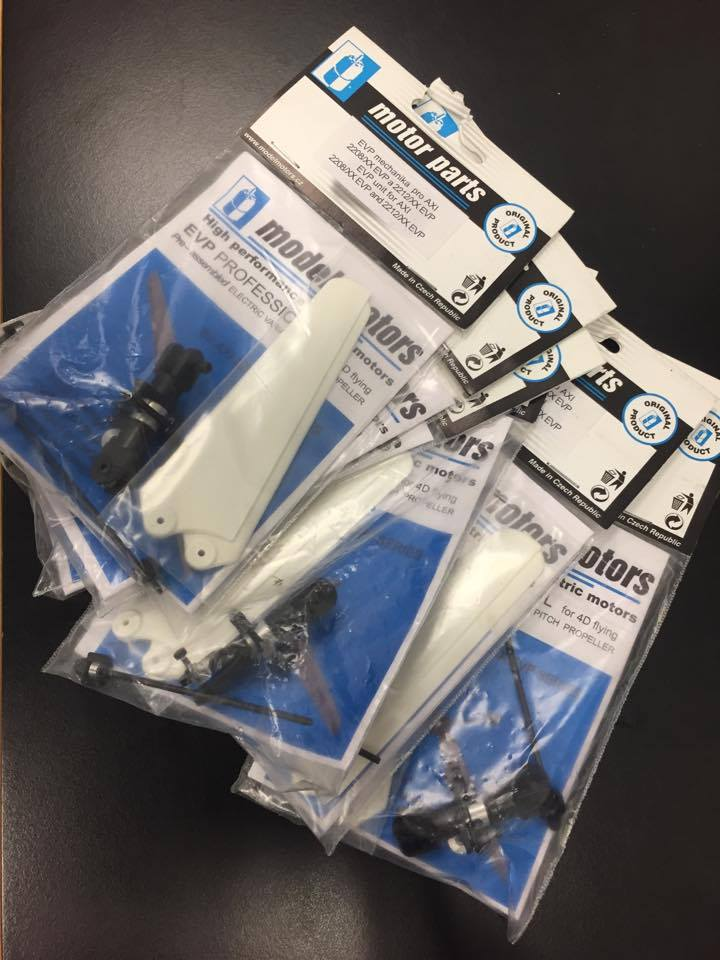
\includegraphics[width = 1\textwidth]{VAPIQ-PICTURES/axievp}
              \caption{Axi Electric Variable Pitch Unit}
            \label{fig:evp}
        \end{minipage}
        \hfill
        \begin{minipage}[b]{0.4\textwidth}
            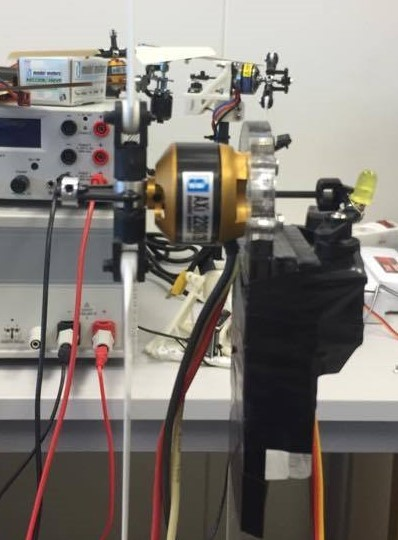
\includegraphics[width = 1\textwidth]{VAPIQ-PICTURES/axi2208}
            \caption{Axi 2208/26 EVP Motor}
            \label{fig:aximotor}
        \end{minipage}
\end{figure}

The team has made improvements in the flight controller code. After running tests, it was discovered that the IMU works well until the propellers are mounted. When additional vibrations are introduced by the propellers, the IMU gives unstable readings. The team had to filter sensor data, and reduce the noise. To mechanically reduce vibrations, rubber gaskets have been mounted under the motors and the IMU has been placed on vibration dampening material within a box. \bigskip

\clearpage

In Qualisys, the team had trouble with the order data was sent. The first measured position was given when the needed position was the most recent. To solve this multi-threading was used, one process collects the newest information and another calculates the desired angles. \bigskip

Additionally, all necessary hardware for the variable pitch quadcopter has been acquired and the motors have been tested for thrust at different pitch angles. The most efficient angle found at the given rotational speed was approximately 6-7 degrees, and more tests will be performed. Vibrations have been reduces to +-5 degress at worst, code has been written for one axis and two axis VPQ.  \bigskip

At the end of Sprint 5, a carbon fiber sandwich frame was made at the composites laboratory at HSN and assembled with the new motors. Denne teksten skal ikke være her :)

\begin{figure}[H]
    \centering
         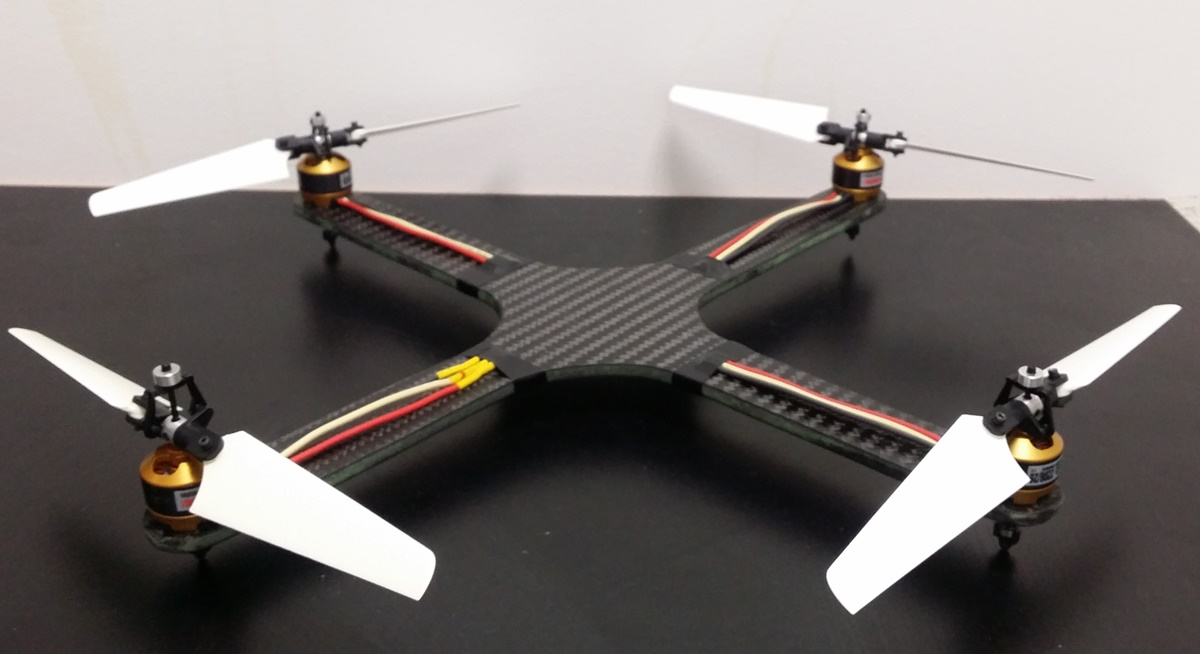
\includegraphics[width = 1\textwidth]{VAPIQ-PICTURES/VariablePitchFrame_Motor}
      \caption{Variable Pitch Frame And Motors }
    \label{fig:vpqframe}
\end{figure} 

\clearpage
\section{Completion and Scope Change}

In sprint 5, 93\% of planned tasks were completed and there was no changes in scope. 

\textbf{Project plan status, Sprint 5:}

\begin{itemize}
        \item Prototype, Variabel Pitch, \textbf{Done}
        \item Flight Testing And Control, \textbf{In Progress}
        \item Servo Control, Variable Pitch, \textbf{Done}
        \item Control System, \textbf{Done}
    \end{itemize}


\begin{figure}[H]
    \centering
         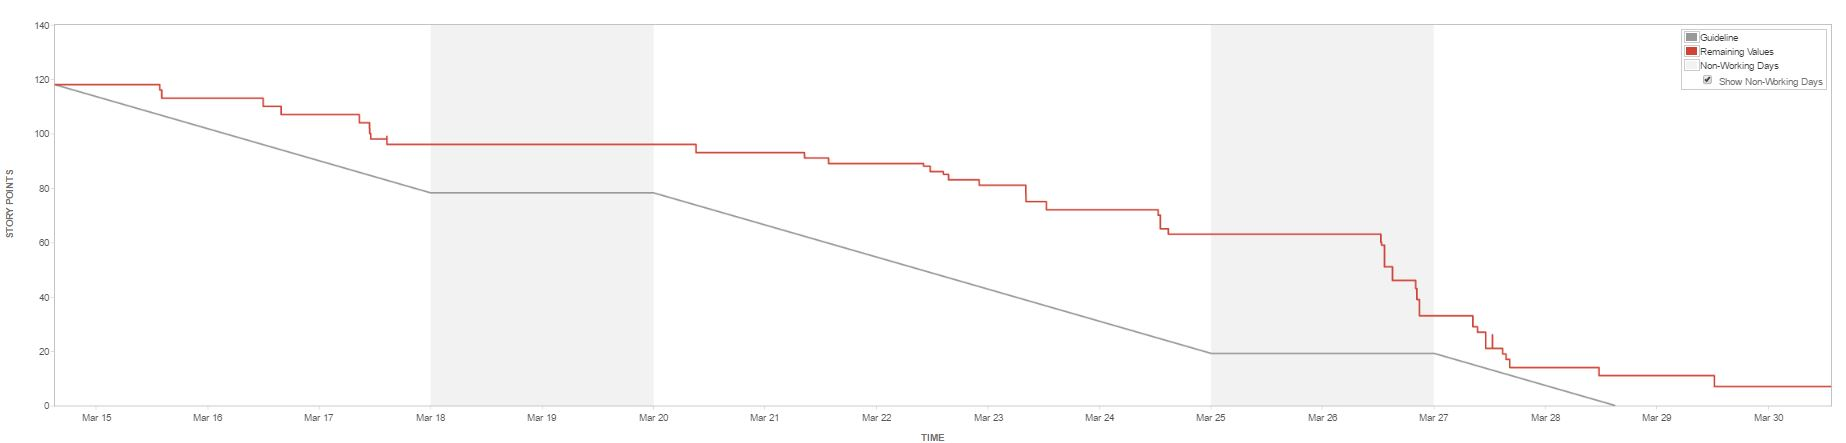
\includegraphics[width = 1\textwidth]{VAPIQ-PICTURES/BDSprint5}
      \caption{Sprint 5 - Burndown Chart}
    \label{fig:bds5}
\end{figure} 


%\subsection{Results and Conclusions}
%prosjektplan



\begin{comment}


Sprint 5:
Scrum Ceremonies
Manually Scheduled	Mechanical Design Review 
Mechanical Improvements
Flight Testing And Control
Servo Control, Variable Pitch
Controller
Advanced Control Functionallity 
Acceptance Testing


Ting å få med:

-V-pitch Rig
-Noise!!!! Noise!!
-Mechanisms did not work-> new plan
-New machanisms from deep in the basment of rc dude in Son0


  \begin{itemize}
        \item Prototype, Variabel Pitch, \textbf{Done} (Mechanisms produced to little thrust and quadcopter was to heavy)
        \item Matlab and Simulink Simulation, \textbf{Postponed}
        \item Stabilization And Regulation, \textbf{In progress}
        \item Tweak Flight Controller, Fixed Pitch, \textbf{In progress}
    \end{itemize}


Manually Scheduled	Control System	11 days	Tue 14.03.17	Tue 28.03.17		
Manually Scheduled	Flight Testing And Control	11 days	Tue 14.03.17	Tue 28.03.17		
Manually Scheduled	11 days	Tue 14.03.17	Tue 28.03.17		
Manually Scheduled	Prototype, Variabel Pitch	17 days	Sat 18.02.17	Mon 13.03.17		

\end{comment}